\newcommand{\specname}{ETIMER}
\newcommand{\status}{Beta}
\newcommand{\ecn}{NA}
\newcommand{\revdate}{2014-03-03}
\newcommand{\rev}{000}
\newcommand{\res}{PB1}
\newcommand{\relay}{PB2}
\newcommand{\startA}{PB3}
\newcommand{\startB}{PB9}
\newcommand{\tresetA}{PB4}
\newcommand{\tresetB}{PB4}
\newcommand{\meterA}{PB6}
\newcommand{\meterB}{PB7}
\newcommand{\timeA}{PC0}
\newcommand{\adjA}{PC1}
\newcommand{\timeB}{PC2}
\newcommand{\adjB}{PC3}
\newcommand{\white}{PC3}

\documentclass[dvips,12pt]{article}
\renewcommand{\contentsname}{3. Index} 

\usepackage{amsmath}
%\usepackage{program}
\usepackage{a4,color,graphics,palatino,fancyhdr}
\usepackage{lastpage}
\usepackage{fancyhdr}
\usepackage{changepage}% http://ctan.org/pkg/changepage
\usepackage{graphicx}
\usepackage{float}

\floatstyle{ruled}
\newfloat{program}{thp}{lop}
\floatname{program}{Source Code}

\setlength{\headheight}{15pt}

\setcounter{secnumdepth}{1}
\setcounter{tocdepth}{1}

\lhead{\specname}
\rhead{rev.\  \rev} 
\chead{\revdate}
\cfoot{\footnotesize Page\ \thepage\ of \pageref{LastPage}}
\pagestyle{fancy}
\title{``F-stop'' enlarging timer with white-light control}

\author{chaz}

\begin{document}

\frenchspacing


\section{Purpose}
Documentation for etimer, microcontroller program to drive a photographic enlarger timer

\tableofcontents
\listoffigures

\newpage
\section{Features}
\begin{itemize}

\item Runs on cheap, common hardware (AVR microcontrollers) with out-of-the-box configuration
(no crystals, fuse bits or bootloaders needed)
\item Runs on readily-available 5V supply (think USB cell phone charger)
\item Measures exposures in units of $log_{2}T$ like God intended
\item Dual-channel for split-grade printing
\item White-light controller which corrects white light source for enlarger head height
according to inverse square law


\end{itemize}


\section{Microcontroller hardware}

The microcontroller used is an ATMEGA328 8-bit AVR\textcopyright\ microcontroller which is widely available for about 3 USFRN in convenient packages. It was selected for its availability in my toolbox. The firmware would run on other AVR microcontrollers with minimal modification. The microcontroller is powered by 5V and runs at 1MHz, which is how it's configured out-of-the-box.  No external crystal is needed, just apply 5V on the Vcc pin and pull up RESET (refer to figure \ref{fig:uc}). Note that if you use a 5V cell-phone power supply, you don't need any voltage regulator.

Flashing this firmware to the microcontroller will require an in-system-programmer such as the AVRISPV2 or USBTinyISP.  Instructions on programming AVR microcontrollers is outside the scope of this document. 

\subsection{Time pots}
Pot 0 sets the exposure time from 0 to 128 seconds on a logarithmic scale. Pot 1 is a fine-adjustment which allows +/- 1 stop of exposure adjustment to be dialed in with resolution of 1/16th stop or less. Thus, setting 8 seconds time on Pot 0 and turning Pot 1 all the way to +1 stop, is the same thing as setting 32 on Pot 0 and dialing Pot 1 all the way to -1 stop. 

\subsection{Meters} 

The use of dials simplifies implementation by combining input and display. However, dials do
not give any feedback as to the progress of the exposure in progress. For feedback the panel meters sweep linearly from full-scale to zero as the exposure progresses. This allows
dodges/burns/filter changes/etc. to be conveniently and repeatably timed and effectively
extends the timer from a 2-channel timer.

\section{White light control}

Non-image, actinic light can be a very useful control. The most convenient place to mount a
white-light source is to the enlarger head. This poses the problem that the white light will
have a different intensity every time you adjust the enlarger head height, according to the
inverse-square law, thus repeatability is difficult to achieve. The white-light output provides
a 16-bit, 8kHz, 5V PWM output which can vary the intensity of the white-light source. AVRs can
directly drive ~10mA loads, or the output can be buffered with a transistor. The adjustment dial can be manually calibrated to one's enlarger. By setting the dial to match the current enlarger-head height, a constant intensity of white light is delivered to the baseboard. 

\section{Perhipheral hardware options}

\renewcommand{\arraystretch}{1.4}% adjust hline heights for prettiness
\begin{figure}[h]
\centering
\begin{tabular}{|c|c|c|c|}
\hline
Input Item&AVR Pin&Voltage details& Function notes\\
\hline
Dial A0&\timeA&0V-5V analog in&set timer A base exposure \\
\hline
Dial A1&\adjA&0V-5V analog in&set timer A fine exposure \\
\hline
Dial B0&\timeB&0V-5V analog in&set timer B base exposure \\
\hline
Dial B1&\adjB&0V-5V analog in&set timer B fine exposure \\
\hline
Button A start&\startA&GND=button pressed&start/stop exposure countdown \\
\hline
Button B start&\startB&GND=button pressed&start/stop exposure countdown \\
\hline
Button A reset&\tresetA&GND=button pressed&start/stop exposure countdown \\
\hline
Button B reset&\tresetB&GND=button pressed&start/stop exposure countdown \\
\hline
Dial W0&\white&0V-5V analog in&set white light intensity\\
\hline
\end{tabular}
\caption{Table Of Inputs}
\label{fig:inputs}
\end{figure}

\renewcommand{\arraystretch}{1.4}% adjust hline heights for prettiness
\begin{figure}[h]
\centering
\begin{tabular}{|c|c|c|c|}
\hline
Output Item&AVR Pin&Voltage details& Function notes\\
\hline
Meter A&\meterA&PWM to panel meter&visualizes exposure \\
\hline
Meter B&\meterA&PWM to panel meter&visualizes exposure \\
\hline
SSR&\relay&Hook to SSR&5V=bulb on\\
\hline
\end{tabular}
\caption{Table Of Outputs}
\label{fig:outputs}
\end{figure}

\begin{figure}[h]
    \begin{centering}
    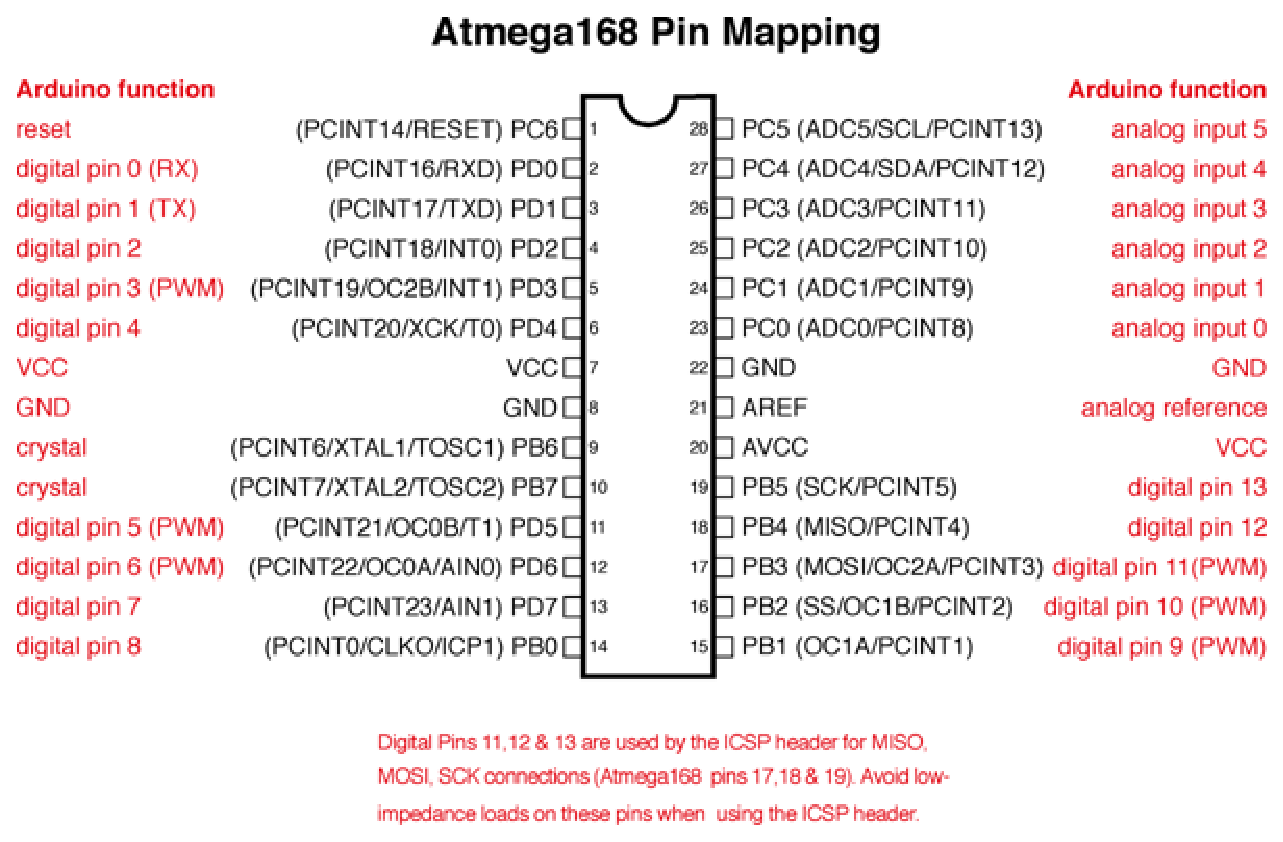
\includegraphics[width=0.8\textwidth]{pins}
    \caption{Pinout for ATMEGA168/328 DIP package} 
    \label{fig:pins}
    \end{centering}
\end{figure}




\centering
\vspace{2cm}
\appendix

\end{document}

